	\documentclass[twoside]{article}
\usepackage{../../estilo-ejercicios}

%--------------------------------------------------------
\begin{document}

\title{Ejercicios de Topología Algebraica}
\author{Javier Aguilar Martín}
\maketitle

\begin{ejercicio}{1}
Probar que para todo $p\geq 0$ se tiene 
\[
C_p(K;\Z)\cong Z_p(K;\Z)\bigoplus B_{p-1}(K;\Z)
\]
y deducir 
\[
C_p(K;\Z)/B_p(K;\Z)\cong H_p(K;\Z)\bigoplus B_{p-1}(K;\Z)
\]
\end{ejercicio}
\begin{solucion}
Tenemos la sucesión exacta corta
\[
0\to Z_p(K;\Z)\hookrightarrow C_p(K;\Z)\xrightarrow{d_p} B_{p-1}(K;\Z)\to 0.
\]
Todos los grupos que aparecen son libres abelianos, bien por definición en el caso de $C_p(K;\Z)$, bien por ser subgrupos de un grupo libre abeliano en los otros dos casos. Por tanto, esta sucesión exacta corta escinde (para grupos libres abelianos se demuestra de forma idéntica al caso de espacios vectoriales). Así que concluimos que 
\[
C_p(K;\Z)\cong Z_p(K;\Z)\bigoplus B_{p-1}(K;\Z).
\]

Ahora, como $B_p(K;\Z)$ es un subgrupo de $Z_p(K;\Z)$, al hacer el cociente deducimos
\[
C_p(K;\Z)/B_p(K;\Z)\cong Z_p(K;\Z)/B_p(K;\Z)\bigoplus B_{p-1}(K;\Z)=H_p(K;\Z)\bigoplus B_{p-1}(K;\Z).
\]
\end{solucion}

\newpage

\begin{ejercicio}{2}
Calcula los grupos de homología simplicial del complejo siguiente
\begin{figure}[h!]
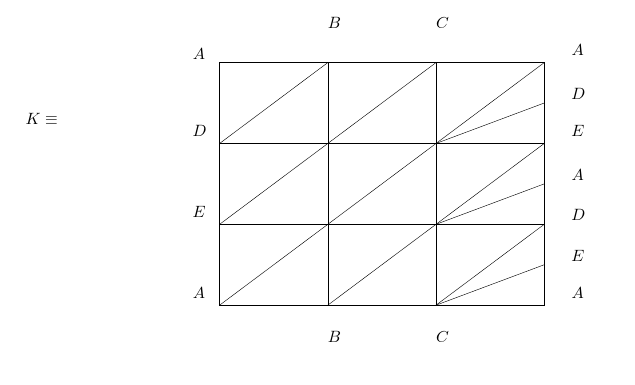
\includegraphics[scale=0.9]{K}
\end{figure}
\end{ejercicio}
\begin{solucion}
En primer lugar, como el complejo es conexo por caminos, sabemos que $H_0(K;\Z)\cong\gene{A}\cong\Z$. Ahora, escribimos el complejo de cadenas simpliciales. Tenemos que $C_n(K;\Z)=0$ para todo $n>2$ y para $n<0$. $C_0(K;\Z)=\gene{A,B,C,D,E,F,G,H,I}\cong\Z^9$ (le damos a los vértices el orden en el que se han escrito). En $C_1(K;\Z)$ tenemos los siguientes generadores
\[
[A:B],[A:C], [A:D], [A:E], [A:G], [A:H], [A:I],   
\]
\[
[B:C], [B:D], [B:F], [B:H], [B:I], [C:D], [C:E], [C:F], [C:G], [C:I], 
\]
\[
[D:E], [D:F], [D:G], [D:I], [E:F], [E:G], [E:H], [E:I], [F:G], [F:H], [G:H], [G:I],[H:I].
\]
Son 30 elementos, así que $C_1(K;\Z)\cong\Z^{30}$. Por último, los generadores de $C_2(K;\Z)$ son
\[
[A:B:D], [A:B:H], [A:C:E], [A:C:G], [A:D:G], [A:D:I], [A:E:I], [A:E:H], 
\]
\[
[B:C:F], [B:C:I], [B:D:F], [B:H:I], [C:D:E], [C:D:I], [C:F:G], 
\]
\[
[D:E:F], [D:E:G], [E:F:H], [E:G:I], [F:G:H], [G:H:I].
\]
Como hay 21 elementos, $C_2(K;\Z)\cong\Z^{21}$. Así que el complejo de cadenas es isomorfo al siguiente:
\[
0\to \Z^{21}\xrightarrow{d_2}\Z^{30}\xrightarrow{d_1}\Z^9\to 0.
\]
Las matrices de las aplicaciones son demasiado grandes como para escribirlas aquí, pero para que el profesor se quede tranquilo de que sé cómo se calculan, haré por ejemplo una columna de la matriz de $d_1$ y otra de $d_2$. Por definición tenemos $d_1([A:B])=B-A$ por definición, luego la primera columa de la matriz de dimensiones $30\times 9$ sería $(-1, 1, 0,0,0,0,0,0,0)'$. La primera columna de la matriz de dimensiones $21\times 30$ de $d_2$ se obtiene al calcular $d_2([A:B:D])=[B:D]-[A:D]+[A:B]$. Esto se corresponde con la columna que tiene un 1 en la posición 1, un $-1$ en la posición 3 y un 1 en la posición 9 (el resto serían 0). 

Nos vamos a ayudar de SAGE para hacer el cálculo final con las siguientes instrucciones:

\begin{verbatim}
K=SimplicialComplex([['A','B', 'D'], ['A','B','H'], ['A','C','E'], ['A','C','G'],
 ['A','D','G'], ['A','D','I'], ['A','E','I'], ['A','E','H'],['B','C','F'], ['B','C','I'], 
 ['B','D','F'], ['B','H','I'], ['C','D','E'], ['C','D','I'], ['C','F','G'], ['D','E','F'], 
 ['D','E','G'], ['E','F','H'], ['E','G','I'], ['F','G','H'], ['G','H','I']])

K.homology()
\end{verbatim}

Las cuales nos dan $H_1(K;\Z)\cong\Z$ y $H_2(K;\Z)=0$. Claramente $H_n(K;\Z)=0$ para cualquier otro $n$ distinto de los que hemos comentado ya. 
\end{solucion}
\end{document}
